\documentclass[journal]{IEEEtran}


% correct bad hyphenation here
\hyphenation{op-tical net-works semi-conduc-tor}
\usepackage{amsmath}
\usepackage{comment}
\usepackage{booktabs}
\usepackage{subfigure}
\usepackage{xcolor}
\usepackage{listings}
\lstset{
  basicstyle=\fontsize{9}{10}\selectfont\ttfamily,
  numbers=left,
  numberstyle= \tiny,
  keywordstyle= \color{ blue!70},
  commentstyle= \color{red!50!green!50!blue!50},
  frame=single,
  rulesepcolor= \color{ red!20!green!20!blue!20} ,
  escapeinside=``,
  xleftmargin=1.5em,xrightmargin=0em, aboveskip=1em,
  framexleftmargin=2em,
  showstringspaces=false,
  showtabs=false,
  breaklines=true
}
\lstdefinelanguage{Solidity}
{
  morekeywords={contract, mapping, address, uint, private, function, public, if, payable},
  morecomment=[l]{//},
  morestring=[b]"
}


\usepackage{multicol}
\usepackage{lipsum}
\usepackage{mathtools}
\usepackage{cuted}

\usepackage{amsmath}
\usepackage{extpfeil}
\usepackage{mathpartir}
\usepackage[mathscr]{eucal}

\usepackage{hyperref}
\usepackage{cleveref}

\usepackage{CJK}

\crefformat{section}{\S#2#1#3} % see manual of cleveref, section 8.2.1
\crefformat{subsection}{\S#2#1#3}
\crefformat{subsubsection}{\S#2#1#3}

\begin{document}
%
% paper title
% Titles are generally capitalized except for words such as a, an, and, as,
% at, but, by, for, in, nor, of, on, or, the, to and up, which are usually
% not capitalized unless they are the first or last word of the title.
% Linebreaks \\ can be used within to get better formatting as desired.
% Do not put math or special symbols in the title.
\title{Bare Demo of IEEEtran.cls for Journals}
%
%
% author names and IEEE memberships
% note positions of commas and nonbreaking spaces ( ~ ) LaTeX will not break
% a structure at a ~ so this keeps an author's name from being broken across
% two lines.
% use \thanks{} to gain access to the first footnote area
% a separate \thanks must be used for each paragraph as LaTeX2e's \thanks
% was not built to handle multiple paragraphs
%

\author{Michael~Shell,~\IEEEmembership{Member,~IEEE,}
	John~Doe,~\IEEEmembership{Fellow,~OSA,}
	and~Jane~Doe,~\IEEEmembership{Life~Fellow,~IEEE}% <-this % stops a space
	\thanks{M. Shell is with the Department
		of Electrical and Computer Engineering, Georgia Institute of Technology, Atlanta,
		GA, 30332 USA e-mail: (see http://www.michaelshell.org/contact.html).}% <-this % stops a space
	\thanks{J. Doe and J. Doe are with Anonymous University.}% <-this % stops a space
	\thanks{Manuscript received April 19, 2005; revised September 17, 2014.}}

% The paper headers
\markboth{Journal of \LaTeX\ Class Files,~Vol.~13, No.~9, September~2014}%
{Shell \MakeLowercase{\textit{et al.}}: Bare Demo of IEEEtran.cls for Journals}
% The only time the second header will appear is for the odd numbered pages
% after the title page when using the twoside option.
%
% *** Note that you probably will NOT want to include the author's ***
% *** name in the headers of peer review papers.                   ***
% You can use \ifCLASSOPTIONpeerreview for conditional compilation here if
% you desire.


% make the title area
\maketitle

% As a general rule, do not put math, special symbols or citations
% in the abstract or keywords.
\begin{abstract}
	The abstract goes here.
\end{abstract}

% Note that keywords are not normally used for peerreview papers.
\begin{IEEEkeywords}
	IEEEtran, journal, \LaTeX, paper, template.
\end{IEEEkeywords}


\IEEEpeerreviewmaketitle



\section{Introduction}
\IEEEPARstart{T}{his}

% wzy
\section{Data Augmentation}
The original dataset contains 40 micro categories of oracle bone characters, each with 85 samples.
Therefore, we have $40 \times 85 = 3400$ samples in total.
This is barely enough for training a convolutional neural network without overfitting, and we need to apply data augmentation to obtain larger dataset adequate for training.

We first make the following observations.

\paragraph{Observation 1} For each pair of characters in Figure~\ref{fig:sym-across}, we may consider them horizontally symmetric.
Thus we can double the number of samples by flipping characters in one category horizontally to obtain those in another category.

\begin{figure}[h]
	\centering
	\begin{minipage}{0.2\linewidth}
		
\includegraphics[width=0.8\linewidth]{fig/observation-1-1.png}
		
\includegraphics[width=0.8\linewidth]{fig/observation-1-2.png}
	\end{minipage}
	% \hfill
	\begin{minipage}{0.2\linewidth}
		
\includegraphics[width=0.8\linewidth]{fig/observation-1-3.png}
		
\includegraphics[width=0.8\linewidth]{fig/observation-1-4.png}
	\end{minipage}
	% \hfill
	\begin{minipage}{0.2\linewidth}
		
\includegraphics[width=0.8\linewidth]{fig/observation-1-5.png}
		
\includegraphics[width=0.8\linewidth]{fig/observation-1-6.png}
	\end{minipage}
	\caption{Symmetric Samples Across Micro-Categories}
	\label{fig:sym-across}
\end{figure}

\paragraph{Observation 2} For characters in Figure~\ref{fig:sym-in}, they are horizontally symmetric by themselves.
We can flip them horizontally to double the number of samples in these categories.

\begin{figure}[h]
	\centering
	
\includegraphics[width=0.8\linewidth]{fig/observation-2.png}
	\caption{Symmetric Samples in Micro-Categories}
	\label{fig:sym-in}
\end{figure}

To balance the samples in different categories after applying above two methods of data augmentation, we need to also double the number of samples in the rest of categories.
We choose to apply affine transforms to the remaining images.
More specifically, we randomly scale images up/down by 0 to 10 percent, randomly translate the image horizontally/vertically by 0 to 10 pixels, randomly rotate and shear images by -10 to 10 degrees.
The augmented images is with the same categories as the original ones.

Then, we need to introduce more noises into the dataset to allow the model trained on it generalize well.
We apply gaussian blur to original images, randomly strengthen/weaken the contrast in each images, randomly add some gaussian noise to each pixel or one channel of images, and randomly make some images brighter or darker by multiplying channels of images.

Figure~\ref{fig:aug-example} shows an example of the affine augmentation and the noise augmentation.
\begin{figure}[h]
	\centering
	\begin{minipage}{0.2\linewidth}
		\subfigure[Original]{
			
\includegraphics[width=\linewidth]{fig/person_0001.jpg}
		}
	\end{minipage}
	\begin{minipage}{0.2\linewidth}
		\subfigure[Affine]{
			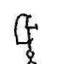
\includegraphics[width=\linewidth]{fig/person_0001_affine.jpg}
		}
	\end{minipage}
	\begin{minipage}{0.2\linewidth}
		\subfigure[Noise]{
			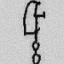
\includegraphics[width=\linewidth]{fig/person_0001_noise.jpg}
		}
	\end{minipage}
	\caption{An Example of Affine Augmentation and Noise Augmentation}
	\label{fig:aug-example}
\end{figure}

When we actually apply the above augmentation methods to images, we first split the dataset into training set and validation set and only apply augment the samples in the training set to avoid data leakage.
We select 10 images from each micro categories to form the validation set.
Eventually, we end up tripling the size of the dataset with 9120 training samples and 400 validation samples.

\section{Character Recognition}
We use two different methods to address the character recognition task for oracle bone characters.
We first learn a deep convolutional neural network to recognize characters, then use the template matching method for the same task.

% wzy
\subsection{Convolutional Neural Network}
The deep neural network for learning the oracle bone characters has the structure in Figure~\ref{fig:network}.

\begin{figure}[h]
	\centering
	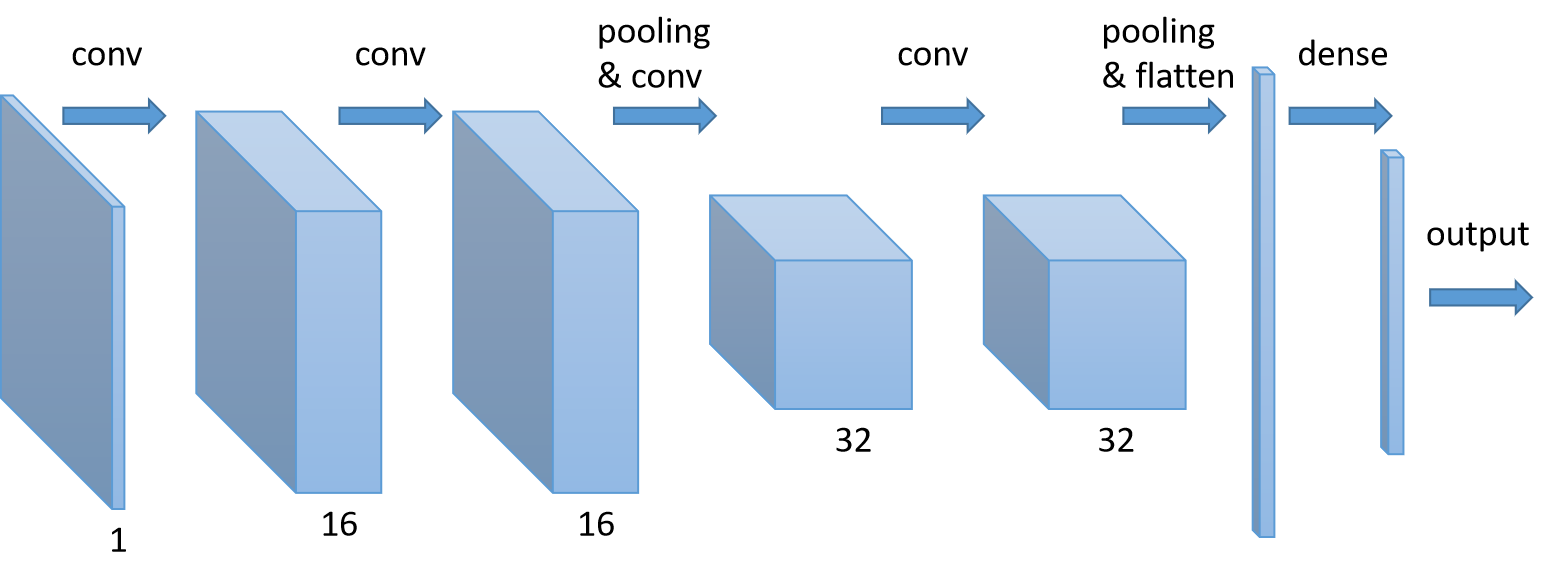
\includegraphics[width=\linewidth]{fig/network.png}
	\caption{Structure of the DNN}
	\label{fig:network}
\end{figure}

The network first uses 2 convolutional layer with 16 filters, then apply max-pooling and batch normalization, then another 2 convolutional layer with 32 filters and pooling layer with normalization. Lastly, it uses one dense layer and an output layer. All trainable layers except the output layer uses ReLU activation and the output layer uses softmax activation.

We use a simple stochastic gradient descent optimizer to train the network on the 9120 training samples and validate it on the remaining 400 samples.

The network for 10 category classification achieves 98\% accuracy on the validation set at the save point, and the one for 40 category classification achieves 88.5\% accuracy on the validation set at the save point.
Figure~\ref{fig:network-confusion} shows the confusion matrix for the validation results.

\begin{figure}[h]
	\centering
	\begin{minipage}{\linewidth}
		\subfigure[Confusion Matrix for 10 Category Classification]{
			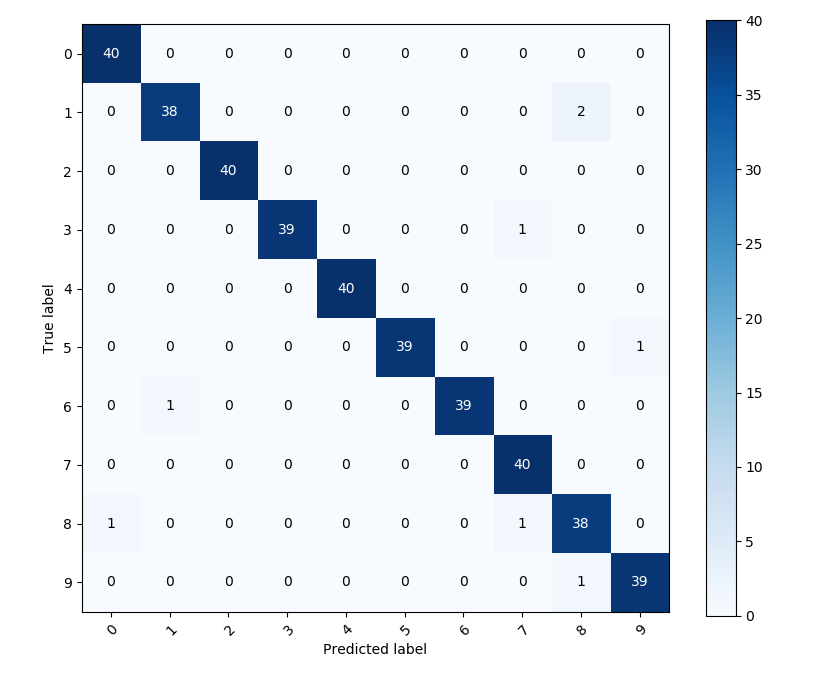
\includegraphics[width=\linewidth]{fig/confusion_oraclenet_conv10.png}
			\label{fig:network-confusion-10}
		}
	\end{minipage}
	\begin{minipage}{\linewidth}
		\hspace{-2em}
		\subfigure[Confusion Matrix for 40 Category Classification]{
			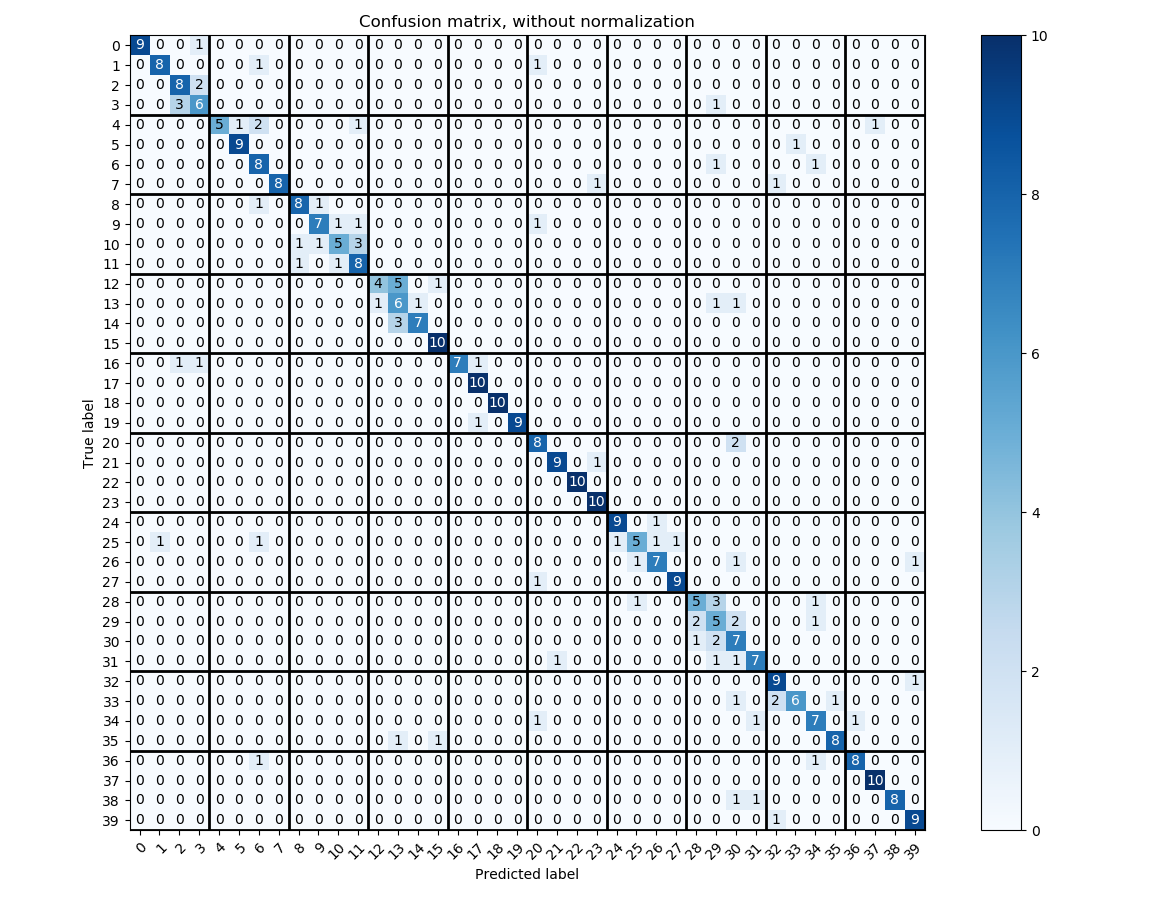
\includegraphics[width=1.15\linewidth]{fig/confusion_oraclenet_conv40.png}
			\label{fig:network-confusion-40}
		}
	\end{minipage}
	\caption{Validation Results}
	\label{fig:network-confusion}
\end{figure}

In Figure~\ref{fig:network-confusion-10}, we can see the classification for 10 macro category is quite accurate, only 7 samples out of 400 is miss-classified.
In Figure~\ref{fig:network-confusion-40}, we use solid lines to separate 10 macro categories among 40 micro categories.
We can see the mistakes made between macro categories is very low and we can use this model for the macro classification task with 98\% accuracy as well.
Most mistakes are made within the macro category.
For example, it miss-classifies many samples for variants of the 3rd and 8th macro categories.

% ljy
\subsection{Template Matching}
% ljy
\subsection{Ensemble of Two Methods}

\section{Experiments}
\subsection{Test Set}
\subsection{Results}

\section{Conclusion}
The conclusion goes here.

\bibliographystyle{IEEEtran}
\bibliography{Ref}


% that's all folks
\end{document}


